\documentclass[10pt,a4paper,headinclude=true]{report}
\usepackage[latin1]{inputenc}
\usepackage[a4paper]{geometry}
\usepackage{a4wide}
\usepackage{amsmath}
\usepackage{amsfonts}
\usepackage{amssymb}
\usepackage{graphicx}
\usepackage{hyperref}
\usepackage{pdflscape} % dlia landscape orientation 
\hypersetup{colorlinks,citecolor=black,filecolor=black,linkcolor=black,urlcolor=black}
\usepackage{float}
\usepackage{setspace}

%\usepackage{biblatex}

\renewcommand{\familydefault}{\sfdefault}

\begin{document}
\onehalfspacing
\title{Industrial Year placement report}
\author{Edgar Ivanov\\ edi@aber.ac.uk \\ \\ IY ICT \& Media Technician}
\date{\today}

\maketitle
\tableofcontents

\chapter{Organization}
My industrial year placement takes place at Aberystwyth University, in Information Services department (further will refer as "IS"). Aberystwyth University is an institution of higher education with research departments, which provides undergraduate and postgraduate education. AU is located in Aberystwyth town, on the west coast of Wales, with average population of 15 thousand people. University was founded in 1872 as University College Wales and has changed its name since then a few times \cite{History}.
The University has 17 academic departments and 27 service departments \cite{Departments} \cite{Departments2}. Most of the teaching departments are located on Penglais campus, as well as in Llanbadarn campus within 15 min. walk from Penglais and in the Old College where Welsh History department and managerial staff are located. There is a big research department called IBERS as well (Institute of Biological, Environmental and Rural Sciences), it used to be an independent organization but then joined the AU. It is located in Gogerddan campus, seven miles away from Penglais, so I had to drive there to do the job required. At the moment there are plans to move some departments to Llanbadarn campus, which was hardly used in the past years, so the University will be even more spread across the different locations.

\section{Information Services}
IS department provides the Library, IT, Management Information and Media Services. There are three main sub-departments: Business Information Systems, ICT \& Customer Support and Library Services within IS (figure~\ref{fig:i-s-hierarchy-tree-march-2012}), each of them is then broken down in to smaller groups and teams that have different roles and responsibilities.

\begin{figure}[H]
\centering
\centerline{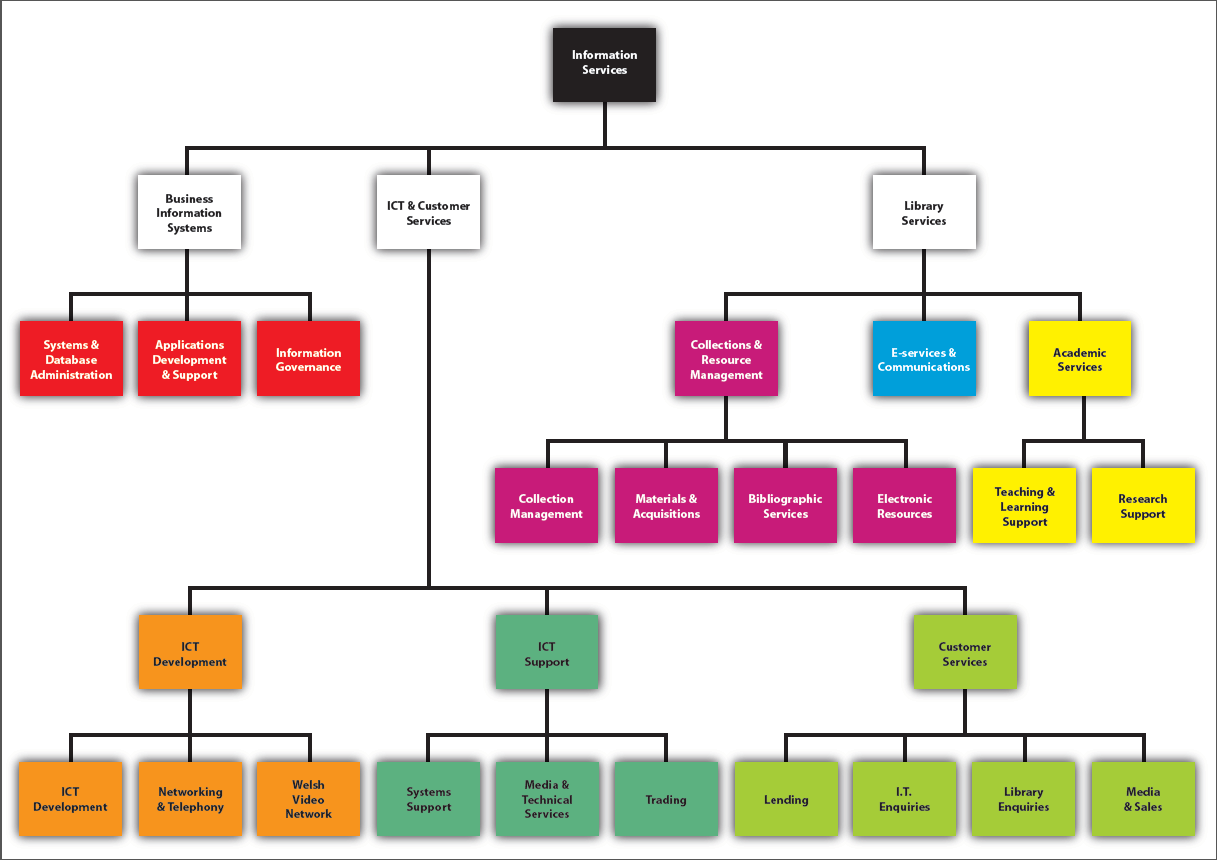
\includegraphics[scale=0.55]{./i-s-hierarchy-tree-march-2012}}
\caption{IS hierarchy tree \cite{ISHierarchyTree}}
\label{fig:i-s-hierarchy-tree-march-2012}
\end{figure}

IS department is located in Hugh Owen building and takes over 40 \% of the E floor.  Figure~\ref{fig:isfloorplan}  represents  IS staff location plan. Most of the IS department employees are based in the open plan office, with the team leaders located in the offices at the edges. My workplace was in the Computer Workshop, which is separated from the main office.

\begin{figure}[H]
\centering
\centerline{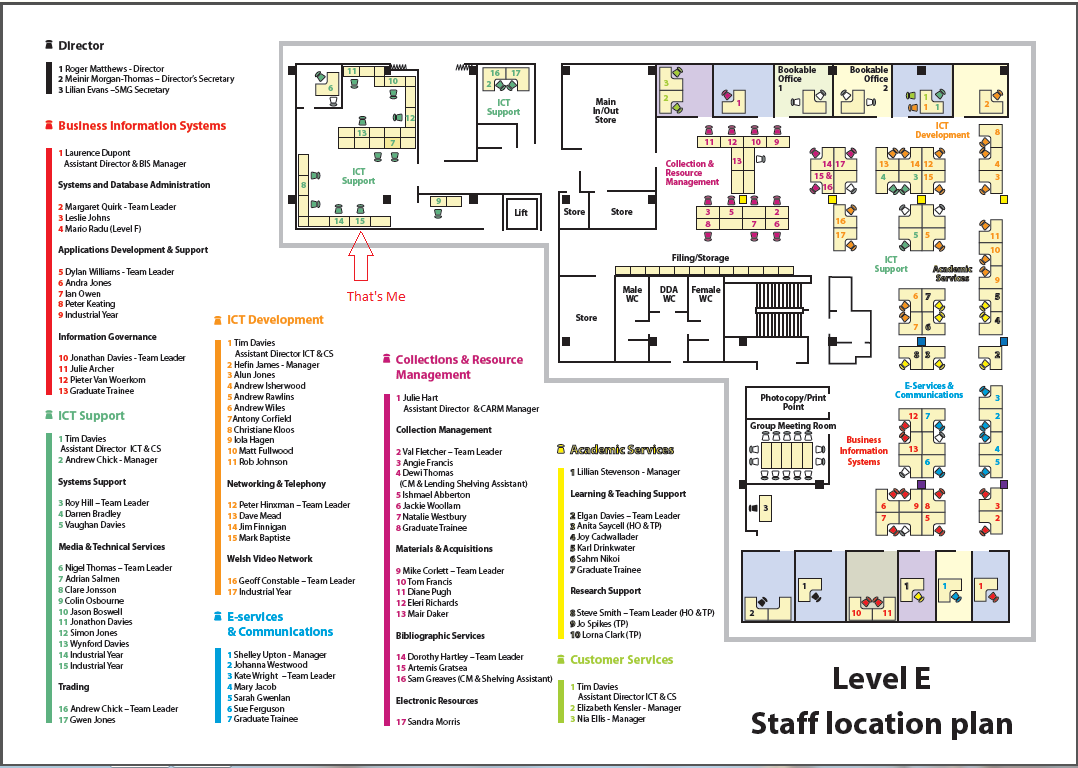
\includegraphics[scale=0.55]{./isfloorplan}}
\caption{IS staff location plan \cite{ISFloor}}
\label{fig:isfloorplan}
\end{figure}

\section{ICT Support}
Whole this group is responsible for ICT equipment provision and support. I will describe sub-teams in detail.
\subsection{Media \& Technical Services (My Team)}
The team that I am based in falls under IS $>$ ICT \& Customer Services $>$ ICT Support and is called "Media \& Technical Services", people in IS usually refer to it as "Workshop". It is defined as a group responsible for the software and hardware upgrades and repairs a wide variety of ICT equipment types. It also provides multimedia services and supports ICT equipment within teaching spaces. All computer relevant hardware repairs are being done here, which includes internal repairs (equipment owned by the University) as well as repairs for external customers (staff, students, members of publicity). The members of this group also provide technical support to the lecturers who experience difficulties with the ICT equipment in the classrooms. 

Computer workshop acts as a second line of contact for the customers and deals with complicated issues that could not be resolved within the reasonable time frame by the help desk staff. IT Enquiries group deals with all incoming phone calls and emails. Usually over 90\% of all enquiries are resolved at this stage. If there is something that requires physical technician presence or problem cannot be resolved remotely or at the help desk, then a staff member opens a new call in our job management system and assigns a job to the appropriate team. That is how workshop team gets most of the jobs. Then the jobs are distributed to the team members by our team leader or technicians pick up the jobs themselves. Jobs that we receive vary greatly from each other, but it is mostly something that requires advanced knowledge in IT, e.g. laptop fix after spillage, the printer that isn't working, slow computer performance, virus removal, delivery and configuration of the new IT equipment, malfunctioning IT equipment diagnostics. Sometimes get unusual jobs and we don't have appropriate equipment or none of us have appropriate qualification to do it. I remember one job when the customer requested to measure signal strength of the antenna, he was then referred to an external company.

There are eight people working in the computer workshop on a permanent basis, one graduate trainee who joined us in January for one year and two industrial year placement students like me, who work on a rotating basis and change every year. Most of the full-timers have relevant education, are A+ certified\cite{A+} and have previous experience in supporting IT. Computer workshop is also certified service provider for Toshiba and Apple Inc. and performs warranty repairs for computers, out of warranty repairs for any other brand computers can be performed here for a charge. 

I would describe Workshop as a relaxed work environment which allows all of us to talk freely to each other whilst remaining focused on our duties and completing assigned jobs. During the first month I was trained by previous industrial year student employees (they left at the end of the first month of my placement to continue their studies), they showed me some systems that we used, helped to deal with my first jobs and provided me with advice. I could seek advice from anybody in the workshop, people were very friendly and helpful, they would explain all I need to do, although not mentioning or skipping some details and I had to find them out myself.
\subsection{Systems Support}
This group is responsible for all the aspects of public service computers, including software licensing, purchasing, management and implementation for IS and many departmental products. It makes backups for most of the University's systems and maintains two main server rooms, one in Penglais and one in Gogerddan. It also provides second/third line software support for the help-desk/workshop.\cite{InternalTeamdescription}
\subsection{Trading}
It offers a wide range of computers, laptops, media equipment and peripherals for sale to University departments, individuals and external customers. Prices are generally competitive and are often at specially negotiated educational terms and/or with extended warranties for the members of the University.\cite{InternalTeamdescription}

\section{ICT Development}
Designs and implements systems and services for IS, other University departments, and external bodies. Also develops, implements, trains and supports IS users on bespoke software and ensures existing systems are efficient and cost effective. This includes Network and Telephone service design promoting standardization and centralization and managing improvements and information security incidents.\cite{InternalTeamdescription}

\section{Customer Services}
Provides Lending, ICT enquiries, Media \& Sales and Library Enquiry services for staff, students and visitors. Monitors the responsiveness and effectiveness of front-line services, ensures services best meet users' needs and promotes awareness of IS enquiry and front-line services. It also manages services and staffing for Fresher's Weekends and students' induction programmes.\cite{InternalTeamdescription}
\subsection{I.T Enquiries}
The first point of contact for face-to-face and online IT enquiries for all IS users. Troubleshoots any problems users experience with accessing or using IS services and resolves them or refers them as appropriate. It also supports the Public printing service, facilitates access to IS services such as email accounts, Aber cards, computing network, and printing and represents users within IS e.g. presenting user feedback at the meetings or user testing new services. \cite{InternalTeamdescription}

A few hours in a week I spent with this team. I am usually staffing help desk where students and staff come with big variety of questions.

\section{BIS and Library Services}
There are also two other sub-departments called "Business Information Systems" and "Library Services". People in BIS are  responsible for the development and support of the systems and processes required to maintain Admissions, Student Records, Finance, HR, Payroll and other associated business functions of the University. Library Services department looks after all the education materials: books, journals, articles as well as after education software systems like "AberLearn Blackboard".\cite{InternalTeamdescription}

\chapter{Customers}
I decided to devote whole chapter to the IS customers since it is essential for the reader to understand who we provide support to. Without customers there wouldn't be IS at all. Here I will describe IS and in particular workshop customers.

Majority of the IS customers are university staff and students of different age, although we occasionally get requests from external bodies or private customers. All customers have different amount of knowledges in IT, sometimes I was finding myself explaining people how to use shortcuts on keyboard efficiently and other basics. The difference in IT knowledge has also required me to treat them differently, since quite a few customers would not understand the terminology I use.  

Computer workshop provides similar service for staff, students and external customers in terms of ICT equipment repairs. If there is a lot of work, priority is usually given to the equipment owned by the University. There is a difference in charge for different customers, equipment owned by University is repaired at smaller hourly rate than the equipment of the external customers.

When a customer drops off his laptop in the workshop or when I collect a broken computer, people want to know how quickly their fault will be fixed and try to be pushy about the time frame in which a fault should be resolved. At the beginning of my placement that was a bit stressful because I tried to satisfy everyone at once promising that their fault would be fixed within 1 to 3 days and then rushing to do the job fast to keep the promise. Impossibility to keep the promise due to overloaded schedule was making my customers unhappy and me frustrated. It had lasted for a while until I have realized the usefulness of the approach and started concentrating properly on one fault instead of trying to fix ten of them at the same time. I discussed the issue with my team leader and have also asked my colleagues to share their experience with me. I am now trying to give a blurred time frame so that the customers would not expect to see their equipment back at least for a few days or a week. 

\chapter{Technical environment}
When I've just started my placement I was amazed by the amount of different software used in IS and how the information was spread across all of these systems. At the beginning I was introduced to the Interzone, Sunrise, Astra, Recall, SharePoint, Aber FAQs, Outlook, Voyager. All of these used to store different kind of information and help people with their day-to-day duties. In this section I will go through technical environment and describe what software and tools I use when doing my job.
  
\section{My Work Environment (Computer Workshop)}
Computer Workshop is an open plan office as shown on ~\ref{fig:isfloorplan} with workbenches , our desks and our team leaders office in the corner (neponiatno). When I've just started my placement I was given a place at the workbench and a computer. In the computer workshop there are tools that you would expect to see in any more or less advanced household, this includes screwdrivers, pliers, soldiering kit, heat gun, drill, hex keys, different types of wrenches. However there are also some specific tools, that are used only for computer hardware diagnostic and repair: power adapters and PSUs (power supply units), PATA and SATA computer data cables, HDD (Hard Disk Drive) cloners, magnifying glass to detect liquid damaged components, all of our workplaces are grounded and have antistatic wrist straps and anti-static mats to prevent electrostatic discharge when working with sensitive computer components, network cable testers, multimeter. We also have a store room to keep new computer components such as new HDDs, cables, monitors, laptop screens, PSUs in case we need any of them during a repair.    

Computer Workshop Technical Environment is probably most unusual in comparison to the rest of the IS. We not only deal with software related issues here, but the hardware as well: soldiering, computer part replacement, cleaning the equipment after spillages, equipment shifting, hardware diagnostics, all unusual jobs come here. I will further describe the tools and techniques that I use most of all. 

When a term starts we tend to get quite a lot of laptops that fail to boot in to the OS. Usually it is caused by damaged HDD, having broken sectors that cannot be read. In such cases Diskology Disk Jockey PRO hard disk cloner\cite{DiskCloner} becomes extremely useful since it can skip broken sectors, filling them with zeros on the destination drive and making it possible to copy the data from the source drive. Some files may become damaged, but this is still better than the frozen OS when it is impossible to copy any data at all. We also tend to get requests to restore lost data from USB pen drives and SD flash cards - then we use R-Studio, a program which performs the scan of the whole drive and then displays all the data that is available for recovery. 

Symantec Ghost is a disk cloning program, capable of making one-to-one copy of any storage media (HDD, SD Card, USB Pendrive). It can also copy one partition from the HDD as well as save disk/partition image as a file. Symantec Ghost is used heavily during MS Windows OS deployment on public computers. After reference Windows installation is complete and all the necessary programs are installed, the whole HDD is being captured in to the file, then computers join multicast session and the image  that has been captured before is applied to all of the machines. It is a very effective technique, because there is no need to spend hours with each computer installing Windows with all the corresponding applications. Usually we deploy the image to 50-100 computers in one go, the size of the image is around 50 GB(that is MS Windows 7, with almost 200 applications required for education use) and that is when Symantec Ghost multicast ability becomes useful, data is sent from one source to all the computers simultaneously in a single transmission and does not overload our network. Usually a public PC is ready for use in 5-12 hours after deployment starts (depends on local network speed).

To remove viruses from the computers we use Sophos Endpoint Antivirus and Microsoft Security Essentials, both of these applications proved to be effective.
 
\section{Interzone}
Interzone is a front end web interface for the database that is used to manage records of the network equipment in Aberystwyth University. It contains comprehensive information about the device including information about the owner. All network equipment connected to the University network has its MAC address registered in our database, otherwise our DHCP server will not assign IP address to the device and without the IP address a device will not be able to use our network facilities.

It is possible to specify search criteria and look for devices that match request on the main interzone. Some of the search criteria are: IP address, MAC address, Owner's login, computer name. On the figure ~\ref{fig:main_interzone_page} you can see the main Interzone page.

\begin{figure}[H]
\centering
\centerline{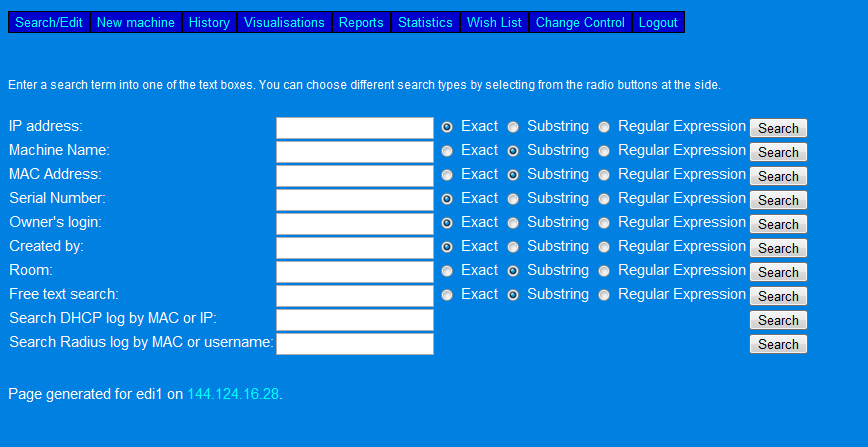
\includegraphics[scale=0.5]{./main_interzone_page}}
\caption{Main Interzone Page}
\label{fig:main_interzone_page}
\end{figure}

On the figure ~\ref{fig:machine_record} Interzone record of my computer.

\begin{figure}[H]
\centering
\centerline{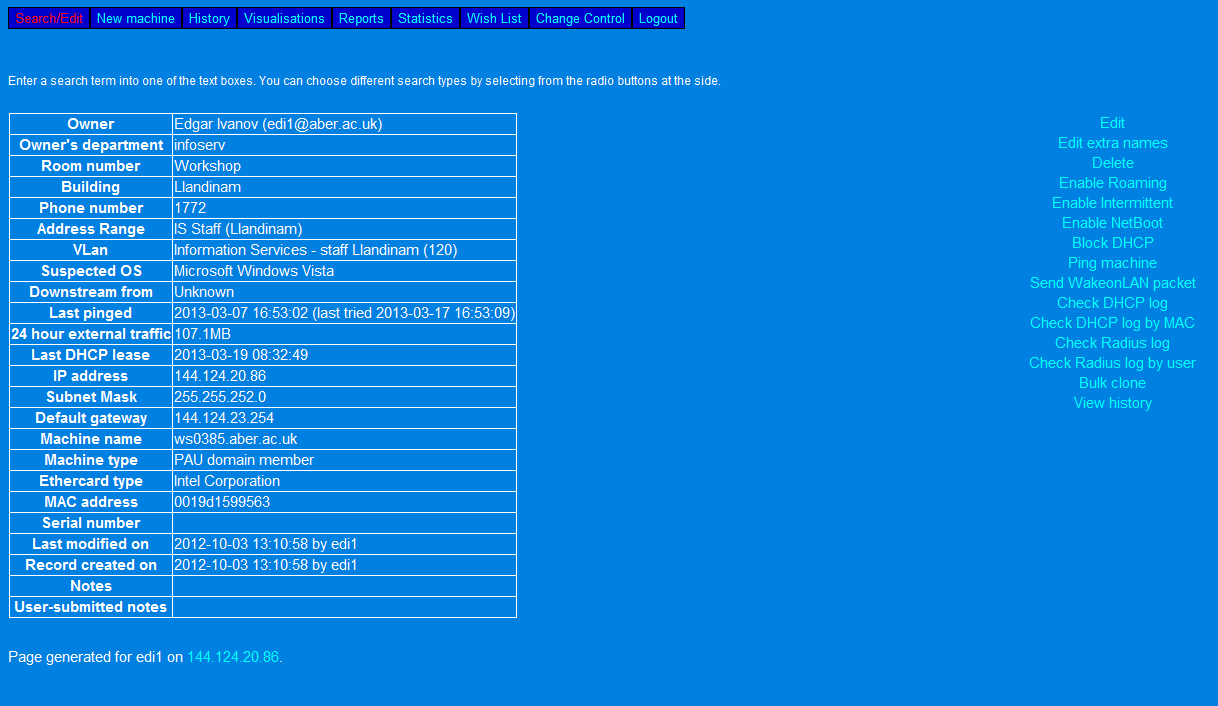
\includegraphics[scale=0.5]{./machine_record}}
\caption{Machine record}
\label{fig:machine_record}
\end{figure}

It contains various information about the owner, owners department, telephone number (if there is one), VLAN, IP and MAC addresses, type of the device (PC, laptop, switch). There is also information about the person who created this record and when it was modified last.

\begin{figure}[H]
\centering
\centerline{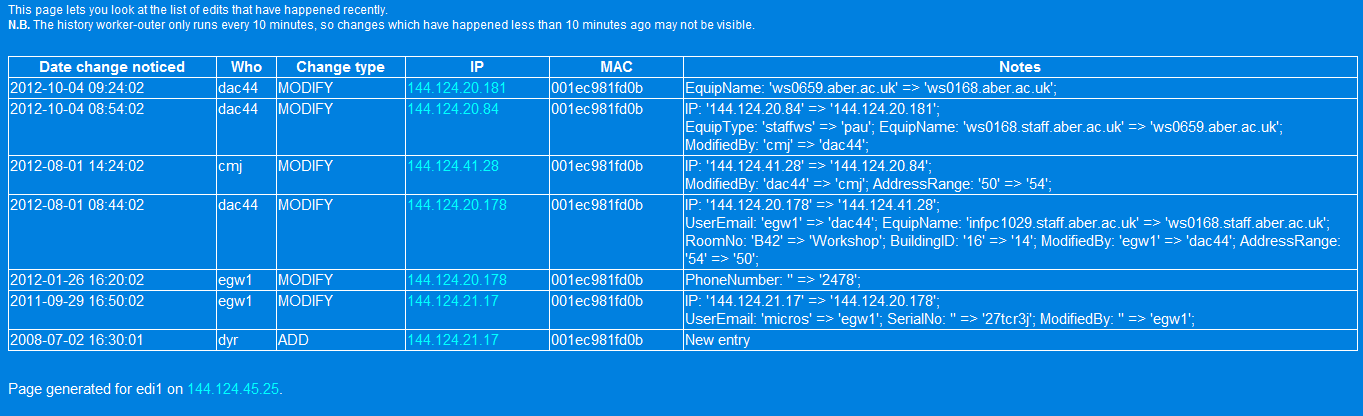
\includegraphics[scale=0.5]{./modification_history}}
\caption{Modification History}
\label{fig:modification_history}
\end{figure}

The information gathered from Interzone can be very useful when troubleshooting computer connection issues. It is possible to check DHCP log to see if the computer gets IP address, look at the RADIUS logs that contain information about the user being successfully or unsuccessfully authenticated in our system. Figure ~\ref{fig:interzone_radius} shows RADIUS log for my mobile phone, it is possible to see that my phone was unable connect to the network due to the authentication problem at some point (I have intentionally changed the password to the wrong one). When working on the help desk and troubleshooting devices which were not connecting to the network properly, Interzone logs let me know what was going wrong so that I could choose an appropriate solution. 

\begin{figure}[H]
\centering
\centerline{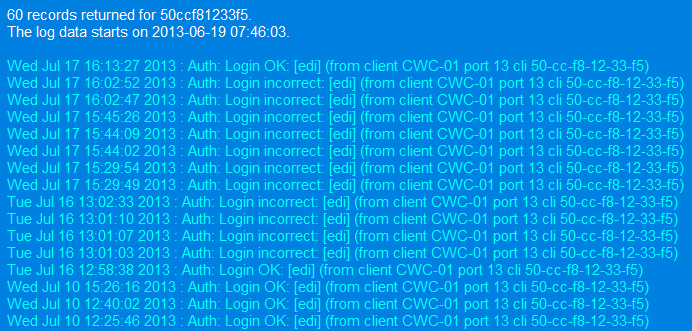
\includegraphics[scale=0.5]{./interzone_radius}}
\caption{RADIUS log}
\label{fig:interzone_radius}
\end{figure}

Interesting reports are generated from the information contained in the database, one of them is on the figure ~\ref{fig:interzone_statistics}, showing the total amount of records in the database (that is pretty much how many physical devices are using University network).

\begin{figure}[H]
\centering
\centerline{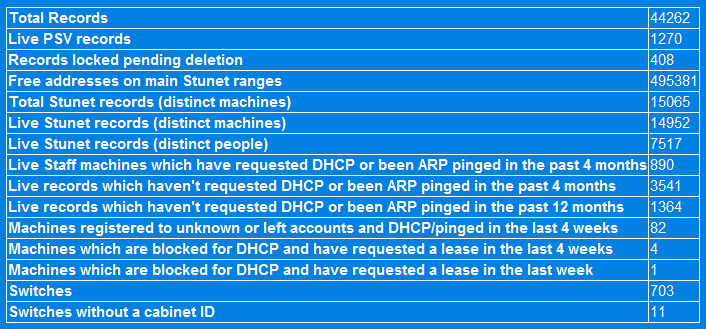
\includegraphics[scale=0.5]{./interzone_statistics}}
\caption{Interzone Statistics}
\label{fig:interzone_statistics}
\end{figure}

\section{Sunrise}
Sunrise is another front end web interface for the database that I use to keep track on current and past calls. This job management system is used to create new "jobs", allocate them to the technician or to the team, add the comments about the job, send emails to the user with updates etc. Almost all the jobs are coming to the Workshop from the help desk, when first line fix is not possible the request is created with necessary information filled in. After the job is assigned to my team our team leader redirects them to the technicians or technicians pick up a job themselves, which happens far more often. On the figure ~\ref{fig:sunrise_main} there is main Sunrise page, with all ongoing jobs assigned to me. There are boxes where you can specify the search criteria and look for the specific job.

\begin{figure}[H]
\centering
\centerline{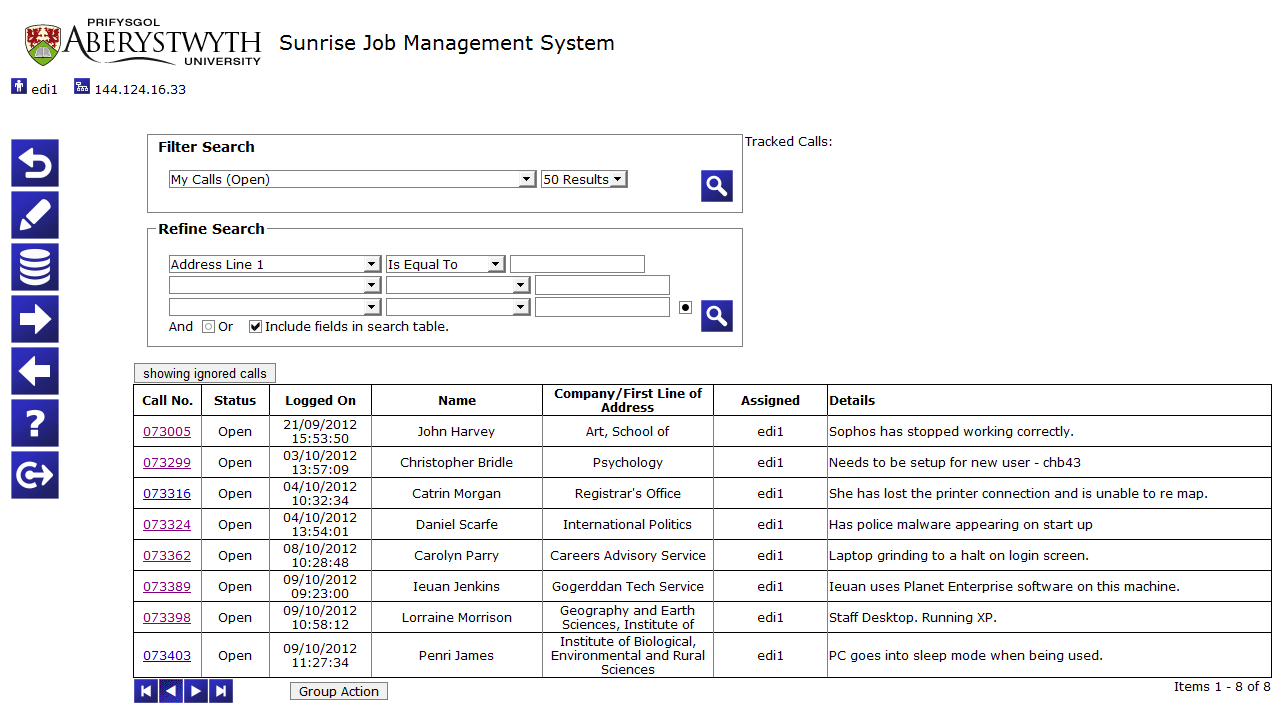
\includegraphics[scale=0.5]{./sunrise_main}}
\caption{Sunrise Main Page}
\label{fig:sunrise_main}
\end{figure}

Figure ~\ref{fig:sunrise_search} shows all the jobs that contain my email address "edi1" in them.

\begin{figure}[H]
\centering
\centerline{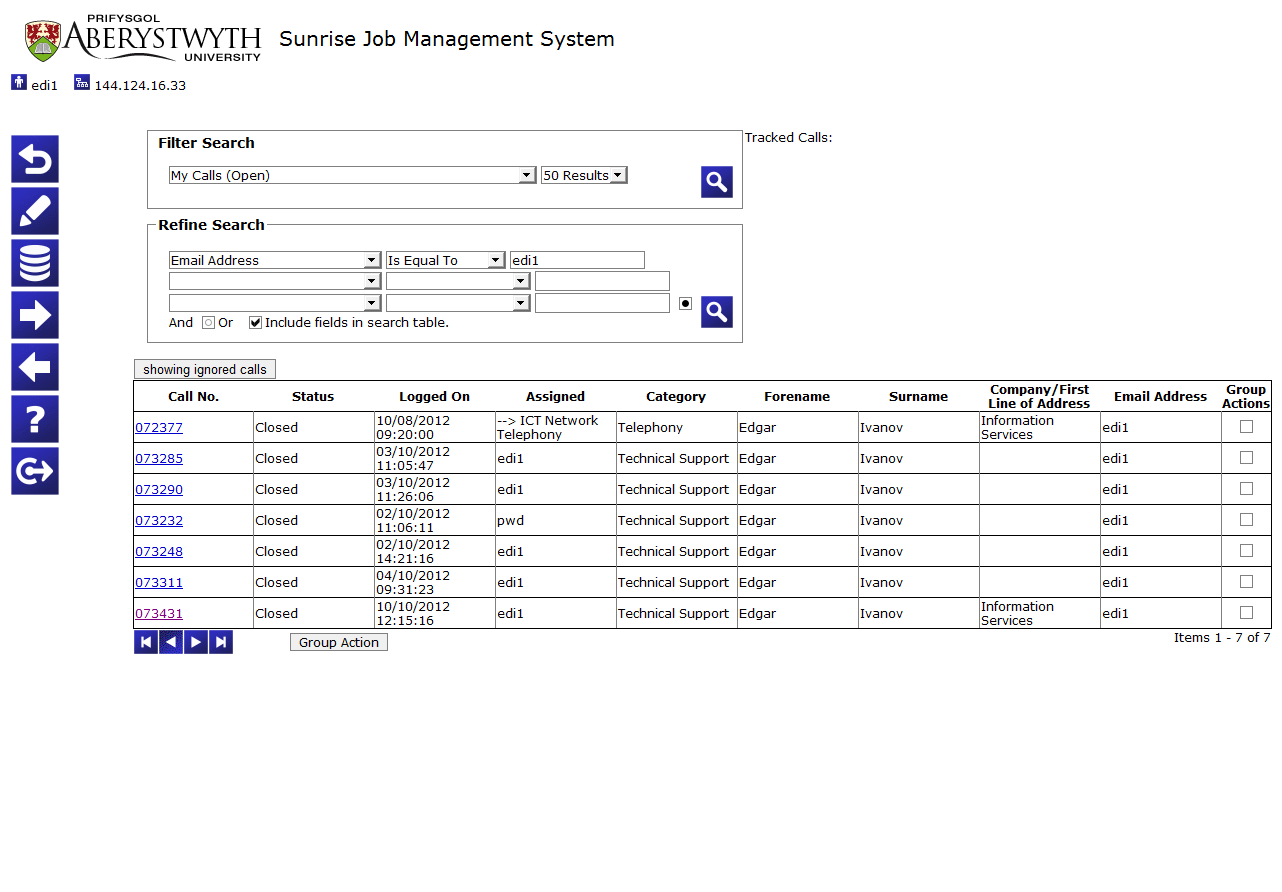
\includegraphics[scale=0.4]{./sunrise_search}}
\caption{Sunrise Search}
\label{fig:sunrise_search}
\end{figure}

Figure ~\ref{fig:sunrise_job} represents a job to be completed. Each job has a unique Call Number, which is 075028 in this case, it also has the email address of the person the job was opened for, his phone number, address, equipment serial number, equipment description (laptop, desktop PC, projector, printer) and any comments where a fault or an issue is described. On the right hand side there is job history pane, each action that technician performs must be added to the history, it helps others to see what was done so far or is planned to be done. Some equipment comes to the workshop more than once and it may be handy for the technician to see what was done in the past.

\begin{figure}[H]
\centering
\centerline{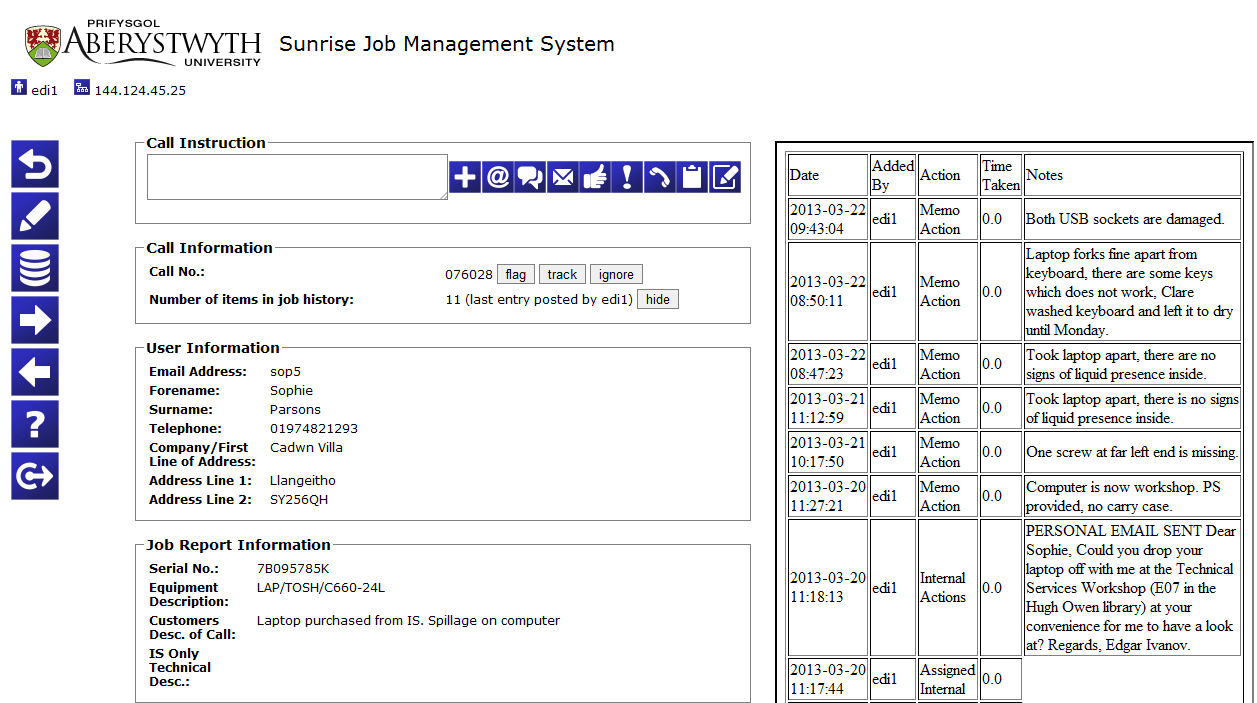
\includegraphics[scale=0.5]{./sunrise_job}}
\caption{Sunrise Job Record}
\label{fig:sunrise_job}
\end{figure}

\section{REG}
Whenever somebody becomes a part of the University (students, staff, visiting staff) a user account is created for them. Username is allocated by the system and usually consists from three letters and some digits if required, for example mine is "edi1". Users then can use them to access their emails, e-journals, manage records about themselves and login to all the systems in the University (if they have access to them). We have web interface called REG to help us manage the accounts. I was mainly using it for unlocking the user accounts while working on the help desk, issuing new passwords, verifying identity of the people at the desk. One of the options I had was to make temporary password for any user, so that I could use their login if required. It was quite useful when I needed to migrate user profile folder on Windows OS and user was away or it was not feasible for them to come in the workshop. In such cases I would create temporary password, login on the computer using their credentials (that is when Windows creates an actual folder for the user together with the other corresponding registry entries), log off and revert the password back. I could then copy all the files from the one machine to the another and be sure that everything will work after the machine is delivered and user logs in.
\section{SNMPc network manager}
Aberystwyth University is a large organization, having thousands of devices connected to its network. To be able to provide reliable service to the end users we need to ensure that our network functions properly and issues are fixed as soon as possible. Network equipment such as: computers, printers, IP cameras, SALTO locks, wireless access points, VoIP phones all relay on ability to communicate (send/receive data), so it is crucial to ensure that there is working network connection at all times.  To monitor all our switches, routers, servers, workstations and printers IS uses a program called SNMPc, developed by Castle Rock Computing. SNMPc is a Distributed Network Manager \cite{SNMPc} that uses SNMP protocol(Simple Network Management Protocol) to communicate and monitor the devices. SNMPc makes it easier to look after the whole network and network devices by identifying unresponsive equipment or network path with the issues and highlighting problematic devices on the network map. 

Figure ~\ref{fig:SNMPc_main} shows a map of our network in SNMPc program. Each icon represents a building, hall of residence or a separate piece of the network, the solid lines between the icons represent fibre optics and thinner lines represent gigabit Ethernet links. Green or purple icon shows that all nodes within are contactable. If an icon turns red it indicates that at least one node in this sub map is not contactable any more \cite{SNPMcSharePoint}. It is enough to give a quick look at the map to identify if there are any issues on the network. I didn't use this application much since there are other people responsible for keeping our network up and running, but I found it quite interesting and useful to look at it from time to time. I can see and explore our network in graphical view, it gives me some understanding of how corporate network should be configured and I will definitely use the knowledge in future.

\begin{figure}[H]
\centering
\centerline{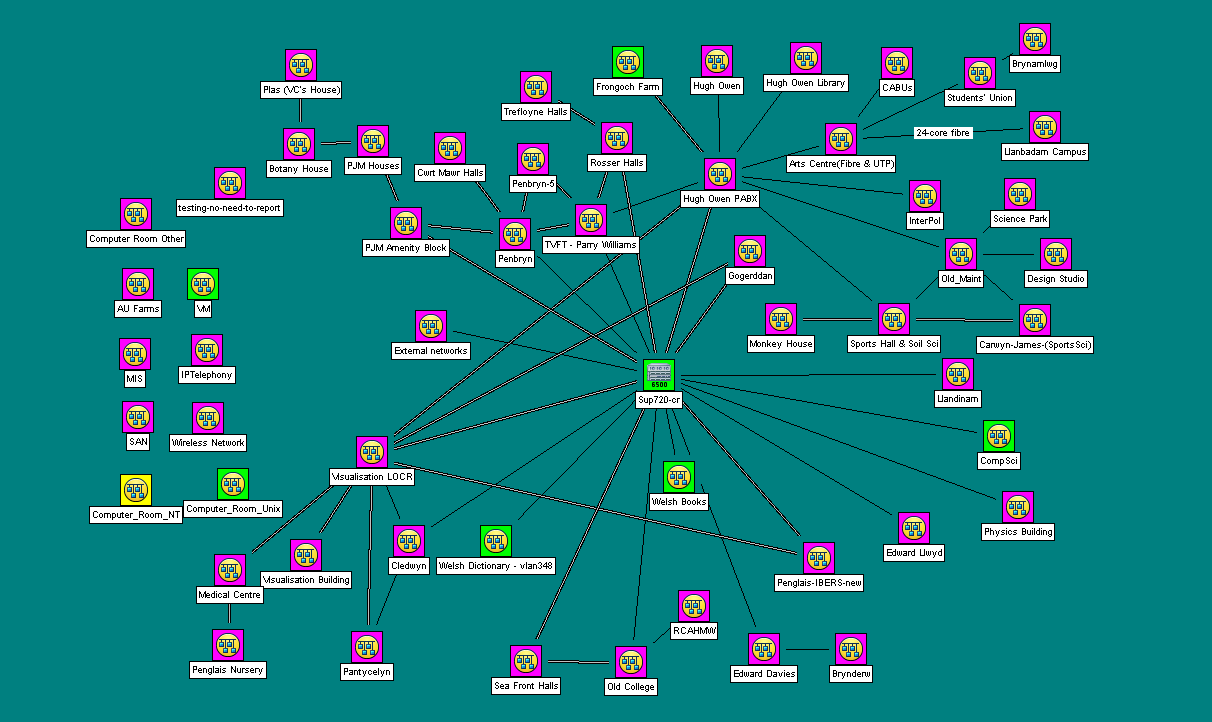
\includegraphics[scale=0.5]{./SNMPc_main}}
\caption{University network map in SNMPc application}
\label{fig:SNMPc_main}
\end{figure}

\section{PCounter}
PCounter is application that allows to  manage user print profiles. It allows to see print balance for everybody in the University, it is possible to increase or decrease balance on the account, see print history and produce reports. I used it mainly for adding money to the user accounts when print credit machine was broken and users were coming to the desk to top up their balance.
\section{VoIP Phones}
Right in the middle of my placement IS finished big project of VoIP phones roll-out in the whole University \cite{VoIP}. VoIP stands for "Voice over Internet Protocol" which means that voice data is carried over the Internet instead of public switched telephone network \cite{VoIP2}. There are numerous advantages of using VoIP phones over the usual ones, VoIP phones can display caller name acquired from the corporate directory, it has extension mobility which means that user can log in to any phone with their credentials, they allow for voice mail to be delivered to the users email inbox. Most of the phones receive power over the Ethernet ("PoE") such approach eliminates the need for a nearby power outlet. When I was on calls in different departments and needed to make a phone call to somebody in the IS I was using feature in the phone that allows to find user phone number by their name. There is also possibility to install "softphone" software on the computer which allows to use computer and internet connection to make telephone calls instead of the usual handset and telephone line \cite{VoIP3}. It is very useful when staff works from home and have to receive phone calls from the colleagues, they are reachable on the same extension number as if they would be in the office. It is also possible to manage all phone aspects remotely with Cisco Unified Communications Manager. For VoIP phones there is no need in dedicated Telephone Exchange equipment, instead all it needs is software running on the server that handles all requests from the phones and manages whole phone infrastructure. 
\section{M drive}
"M" dive is known by the University staff and students as a network file store, where users can keep any kind of information, the same as on USB pen drive and it is accessible from any computer that has access to the Internet. Size of file store is limited to 2 GB per user.  It is very convenient since information is stored on University servers and there is no need to carry any physical media. IS makes regular backups of all "M" drives, so if user deleted something accidentally it is possible to recover file from the backup. When users log in on to the computers in the University computer rooms, filestore is automatically mapped on the computer as "M" drive \cite{MDrive}.

\section{Computers}
Here at Aberystwyth University we have hundreds of computers used across campuses by both staff and students. While computers used by staff members may vary greatly in configuration, all public computers used by the students have the same hardware and software configuration across all campuses.
\subsection{PSVs}
PSVs (Public Service) are computers that can use anybody who have University user account. IS manages around 500 public computers across campuses \cite{PSVs2}. We have two different versions of Optiplex 7010 computers. One model with higher specifications for teaching stations and USFF model for the student use. 

This summer we deployed new USFF Dell Optiplex 7010 \cite{PSVs} computers, since old ones were almost seven years old and didn't match current student and staff needs. New computers are more powerful equipped with Intel i3 processors, 4GB of RAM and 320 GB HDDs. All PSVs run MS Windows 7 OS and are "PSV" domain members which makes their management more easy, there are more than 200 applications installed for academic use on them. A few big rooms with computers in them (from 25 to 100 PCs in one room) are available for teaching purposes and for general use.  
\begin{figure}[H]
\centering
\centerline{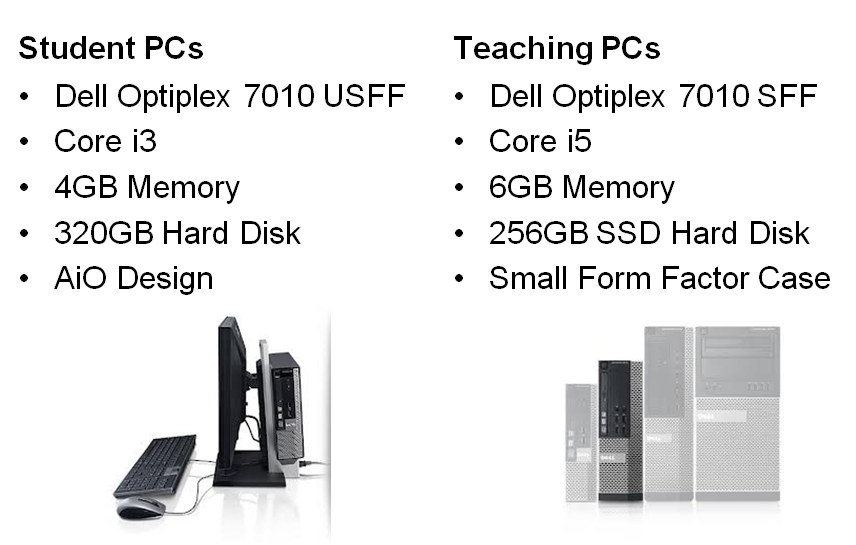
\includegraphics[scale=0.5]{./PSVs}}
\caption{Public workstation PCs \cite{PSVs}}
\label{fig:PSVs}
\end{figure}
\subsection{Staff Computers}
In Aberystwyth University departments are responsible for buying computers to their staff members, money for them are allocated from the departments budget. All such purchases go through IS. After IS is informed of the computer choice, it goes through "build" process, necessary software installed and PC joined to the domain. 

During my placement I was dealing with big variety of the staff computers, most of them were standard tower PCs, with average hardware specifications, suitable for office work. Standard PC would be equipped with Intel Core Duo Processor (which is now more than six years old), from one to two GB of RAM, 80 - 250 GB HDD, integrated video card, running MS Windows: XP, Vista or 7. However across different departments I saw quite a lot of old PCs which were running Windows XP and were hardly dealing with MS Office 2010 applications. Also there were some new Dell Optiplex computers, produced in last few years with quite good specifications.I also saw an old computer running OS/2, it was connected to some research equipment, reason for that one still being used is that there is no new software written for the new operating systems and there is pretty much no choice, you either use it as it is, or not use at all. I have also dealt with wide variety of Apple Macintosh Computers, from low power Mac AirBooks to powerful Mac Pros which were used for image processing. The biggest amount of them (around 30) I saw in geography department, where they were used to process large amounts of data. There is one interesting thing that I have noticed: during the whole year I haven't dealt with any staff computer that would be equipped with AMD processor. It frustrates me since AMD CPUs are cheaper due to competition on the market share between Intel and AMD(my own thoughts).

All in all computers seems to be fine for the purposes that they are used for, however some departments should really consider urgent upgrades. 

\section{Aber FAQs \& Sharepoint}
\label{sec:faqs}
Aber FAQs is database of frequently asked questions, with answers to them. It is available to anybody on Internet and contains useful information on wide variety of questions. I used it mainly to remind myself of how to do certain things like computer connection to the university network, user account activation, email handler configuration etc. There is as well hidden part of this website which contains information only for IS staff. To access it user needs to provide username and password. Information in hidden part is relevant only to IS staff since in contains procedures with step-by-step guide and passwords required to complete tasks. It is organized in the same way as main website, having questions and then answers to them. I used it only a few times, when I had shifts on help desk, to create and activate new society account.

Sharepoint is described by Microsoft as collaboration platform \cite{Sharepoint}. In IS it is used primarily for content and document management. One of the features that I liked about Sharepoint is revision control capability, which allows to view older versions of the same document. Since anybody who has access to the document can change it and then save changes it may be handy to go back in time and see what changes were done and who exactly did them. On Sharepoint IS staff keeps different documents relevant to their work. Some of the Staff Help Desk procedures are kept on Sharepont as well as on Aber FAQs, this is something that is going be changed in future, but nobody knows when it will happen. All Computer Workshop document are kept here as well. 

To provide bets experience for University lecturers workshop staff regularly visits all teaching rooms and checks for all equipment to work, this includes PC, DVD Player, Microphone, Video Camera, Projector, Speakers. After check is completed and everything works, whoever completed the check should update document on Sharepont were data about projector lamp hours is kept. This data is kept to determine how heavily projector is used and if any lamp should be replaced if it reaches end-of-life. Now I would like to describe how this update happens, person opens simple MS Excel spreadsheet, deletes old value and enters new one, then saves document. I personally was terrified by this approach to keep data. It would fine for some newbie at home to keep data in such way, but definitely not in serious organization as University. I would expect to see database, with simple front end, but not this. I saw a lot of such stupid things during my placement and I even get used to some of them so that now I could not even tell which way is right one. What I have learned from this is that sometimes it is useful to look fresh to things that you get used to do.      


\section{PSR2}
Here I would like to write some critics about computer workshop and our team leader as well. We have web application called PSR2 Maintenance where we keep information about computer room layouts with computer serial numbers. It is very simple web interface written with help of php and pulls data from the database. The only concern that I have is that this page is operating from one of the employees "M" drive. University provides such facility for all users to host their own web pages. All user needs to do is upload web site to special folder on "M" drive, change permissions and web site is available for the world. Drawback here is that if user account will be locked web page will not operate, it will display Not Found error message instead. 

On figure ~\ref{fig:main_PSR2_page} you can see main PSR2 page, which contains teaching rooms list that workshop technicians look after.

\begin{figure}[H]
\centering
\centerline{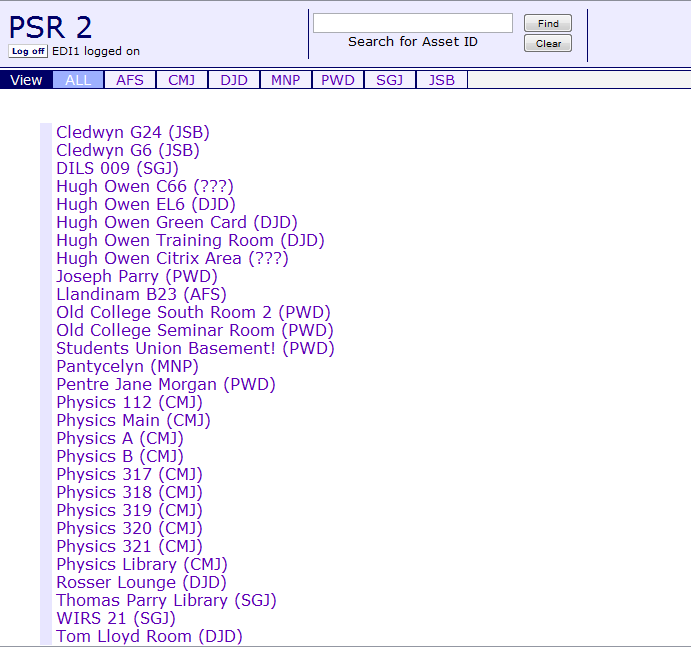
\includegraphics[scale=0.3]{./PSR2}}
\caption{Main PSR2 Page}
\label{fig:main_PSR2_page}
\end{figure}

Figure~\ref{fig:PSR2_SU_Room_layout} shows Students Union computer room layout, with computer names and serial numbers. Room comment holds code to unlock monitors from security straps. It also contains information when each computer was last time checked.

 It contains quite a lot of information, which is crucial to our work, and if for some reason account will be locked we will lose access to that information, which is at my knowledge is not held anywhere else.

\begin{figure}[H]
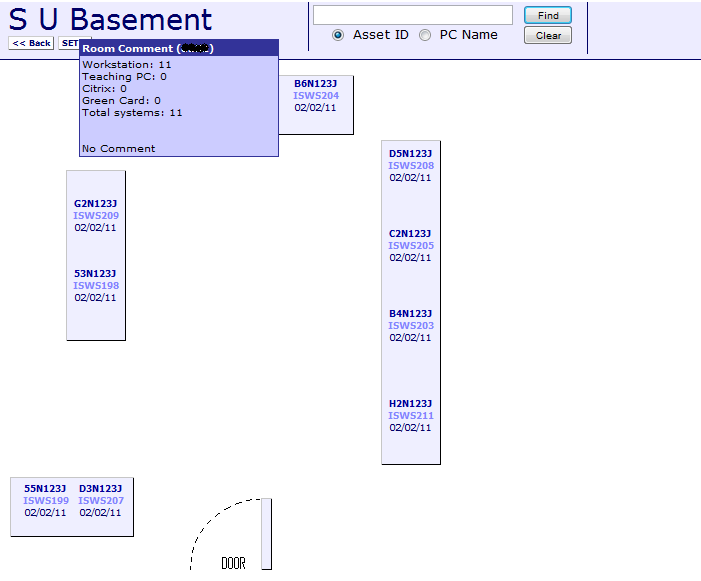
\includegraphics[scale=0.5]{./PSR2_SU_Room_layout}
\caption{PSR2 Students Union Computer Room Layout}
\label{fig:PSR2_SU_Room_layout}
\end{figure}

When I spoke to my college she explained me that this application was written for herself in first instance and then when our team leader accidentally saw it he asked for other workshop members to be added on the user list. That is how sometimes happens, no planning, no testing, no official discussion.
\chapter{What I did}
Describe your 'routine' weekly duties. Spend a bit more time on areas where you have
responsibility or have put in effort e.g. summer builds, FAQS, summer course
registrations, any exploratory projects or mini-projects you may have been given to
name a few.

My work hours are from 8:30 until 17:00 Monday to Thursday and on Fridays we work one hour less, until 16:00. Since I live just a few kilometres away from the university I get to work by walk and it usually takes me around 15 min. In workshop my usual duties are computer room checks, lecturer support in teaching spaces over the phone or if required in personal and what I do most of my time is assigned jobs completion.

My work day starts from assigned jobs review. I open Sunrise - our job management system and look through all jobs assigned to me, then I decide and plan what to do during the day. I also look through our list of unassigned jobs and if there are jobs that I can do I assign them to myself. Usually I avoid taking difficult hardware faults with laptops since officially I don't have appropriate qualification, but I occasionally do screen, HDD, RAM replacement.

When I joined IS I had to attend compulsory trainings for new staff. I was trained how to deal with customers in different situations, introduced to the IS rules and regulations, data protection act. Also received trainings about user data management on reg and AStRA, IS news channels management, Voyager use - university library system. I was also shown how to use and provide support for Abercast, QMP, Qwizdom - these are applications and tools used by lecturers to provide better experience for the students during lectures. I also learned many more other little things while doing jobs and providing support to the customers.

There are two main types of the jobs that I do, those that I can do in the workshop and those were I need to visit customer. After I read fault description I decide whether job can be done on customers site or in the workshop. Usually software faults require physical technician presence since if job appeared in our database it means that first line fix was not available or impossible. With hardware faults everything is much simpler, I just go, pick up faulty equipment and bring to the workshop. With laptops I always send email to the customer asking he/she to bring laptop to the workshop disregarding if it is software or hardware issue. Whether it is simple software problem or some hardware issue I always contact customer and arrange time when I can come and fix problem or pick up faulty equipment. Sometimes software problems may be difficult and after few hours of trying to fix it on site I decide to take computer with me back to the workshop where in more relaxed environment I can look for a fix or ask my colleagues for advice.

\section{Room Checks}
As I have already said in section ~\ref{sec:faqs} we perform room checks to determine any ICT equipment with faults or not functioning properly, we do it a few times during the term time. All permanent employees are responsible for lecture rooms and as it used to be IYs take responsibility over big computer rooms. Usually I performs room checks with my colleague industrial year student, he is in the same position as me. When we perform room checks we log in to each computer in that room, as doing so eliminates problems with keyboard and mouse as well as with network (we use domain user accounts, so OS requires to fetch data from the domain controller over the network and if user account is logged in successfully it means everything is ok). We also check teaching equipment: if microphone works fine, there is sound coming from the speakers, projector works and image is of good quality, DVD player plays movies, check batteries in RCs. Usual problems that we find are unplugged network cables, mouse and keyboard being connected to the different computer, projector settings being changed, power cables unplugged. Rarely we find something more difficult. As far as I remember we had around 4 or 5 public computers out of 500 with hardware faults during the year, broken HDD, RAM, Video Card, Motherboard. 
\section{Lecturer support}
Usually when lecturers struggles with ICT equipment in the teaching space they can pick up phone, which is usually next to the computer, and it automatically dials directly to the workshop. It is everybody's duty in the workshop to pick up such phone call and provide help. I dealt with many such calls, usually people ask help in turning on projector, recording lectures with Panopto (lecture capture software), report microphones which don't pick up any sound or blank screens after turning projector on. I noticed that most of the times it is users fault, they usually don't read notes printed for them and lying next to the computer, since most of the issues with fixes are covered in those sheets. In first instance we try to help user over the phone and give some guidance, if problem still persist we have to go to the lecture room and try fix problem over there. When I just started my placement I used to visit user on each occasion of such calls since I was unable to resolve any problem over the phone, but after a few weeks I learned how all equipment is set up and managed to guide user until issue is resolved. The biggest problem that I face when supporting user over the phone is that I can't see what user sees, user may describe problem in wrong way or miss some important piece of information. I had situations when I was trying to resolve one problem over the phone, but when I turned up to the room I discovered that issue was completely different. I didn't receive any training in this field so I had to develop my own techniques of troubleshooting over the phone and it took me some time to learn to ask right questions. For example if user says that there is no picture on the screen I need to work up from the most obvious reasons to the more complex. I would ask if computer and screen is switched on, if projector is switched on and there are lights coming from it, the last step that I would try over the phone is ask to switch between video inputs (from RGB1 to RGB2) and that is where problem usually is resolved. Such appears appears if user uses their laptop as source of image for the projector and switches input to different cable, as the result when next user comes they cannot understand why there is no picture on the screen. If problem is not resolved over the phone then I go to the lecture theatre personally to see what is wrong, usually I find something very silly like switch which is hidden from the people eyes and with red mar on it "DO NOT SWITCH OF" being switched of.  
\section{Enquiry desk}
Enquiry desk located in Hugh Owen library provides help to the users with library and IT enquiries. I was scheduled to work on help desk twice a week for two hours. It was completely different experience in comparison to what I get used in the workshop. I helped students and staff members with IT related issues, occasional I would handle users with library  questions but it is primarily librarians duty. Usually I would assist users when connecting their laptops or hand held devices to our network, activate user accounts for new students and staff, issue new passwords for those who forgot them, direct people in a right way, take payments for fines and printing credit. Working on help desk gave me better understanding of what issues face front line staff members. I learned useful techniques from them like use of Windows Remote Assistance to solve some of the problems form the workshop instead of visiting user on each occasion.
  
\section{Becoming Mac Technician}
During my placement when I had some free time at work and at home I completed Self-Paced Mac Technician Course and after passing exam I am now holder of "Certified Apple Macintosh Technician" certificate. All fees for exam where paid by IS and all I had to do is study hard. Before completing this course I literally knew nothing about Apple computers and Mac OS X, so it was interesting course and I learned a lot. Now I know that there are differences between simple PCs and Apple computers. 
\chapter{Critical evaluation}

\bibliographystyle{ieeetr}
\bibliography{bibl}

\end{document}